\newpage

\section{Durchführung}
\label{sec:Durchführung}

Die Durchführung basiert auf der gleichmäßigen Erwärmung der Kaliumbromidprobe,
nachdem die internen Dipole ausgerichtet wurden und einer Notation des 
zugehörigen Stroms, der aufgrund der Relaxation der Dipole durch den folgenden 
Versuchsaufbau messbar ist.

\subsection{Versuchsaufbau}

\begin{figure}
    \centering
    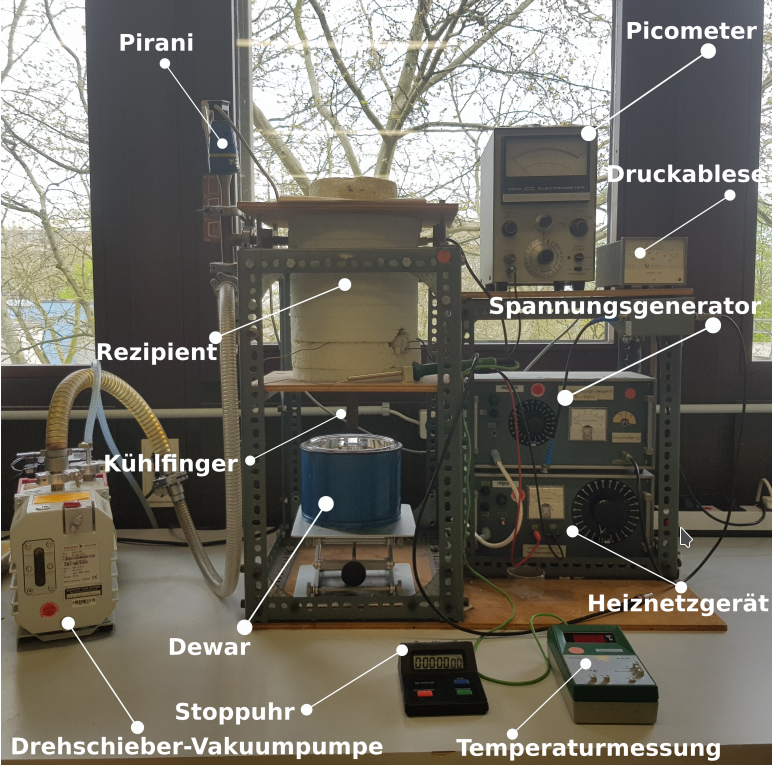
\includegraphics[width=0.8\textwidth, keepaspectratio]{figure/AufbauFoto.png}
    \caption{Auf diesem Foto ist der verwendete Versuchsaufbau abgebildet. 
    \cite{sample}}
    \label{abb1}
\end{figure}

Die Beschriftung der Bestandteile des Aufbaus sind in Abbildung \ref{abb1} dargestellt.
Hauptbauteil der Apparatur ist der Rezipient, ein Plattenkondensator mit der Kaliumbromidplatte
im Inneren, welcher vakuumisiert und isoliert verschlossen ist. 
Zur Temperaturregulation des Ionenkristalls dient lediglich ein Kühlfinger, 
der aus dem Rezipient herausragt und durch eintauchen in ein Bad aus flüssigem 
Stickstoff abgekühlt bzw. in seiner Erwärmung durch die Umgebungstemperatur reguliert 
werden kann. Über die Temperaturvariation am Kühlfinger wird dementsprechend die 
Temperatur der Kaliumbromidplatte kontolliert. 
Außerdem ist ein Heiznetzgerät an dem Rezipient angeschlossen, das eine Erwärmung 
der Apparatur ermöglicht, wenn die Umgebungstemperatur für eine konstante 
Heizrate nicht mehr ausreichend ist. 
Das Ablesen des Stroms, welcher aufgrund der Dipolrelaxation im Kristall zwischen 
den Kondensatorplatten entsteht, wird über ein zugeschaltetes Picometer 
bzw. Amperemeter (Abbildung \ref{abb2}) ermöglicht.
In Abbildung \ref{abb2} ist die Schaltung und der Aufbau im Rezipient strukturiert 
dargestellt. Es ist zu erkennen, dass die Erwärmung durch das Heiznetzgerät 
mittels einer sromdurchflossenen Spule realisiert wird, die um die Probe
verbaut wurde. Außerdem wird deutlich, dass das Thermoelement unmittelbar an 
der Probe verbaut wurde und somit die Temperatur des Kristalls wiedergibt \cite{sample}. 

\begin{figure}
    \centering
    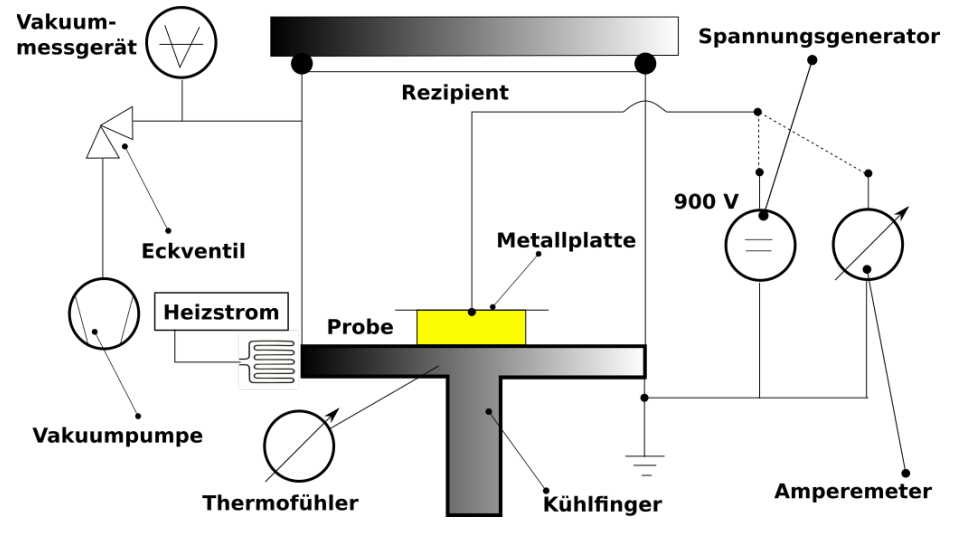
\includegraphics[width=0.8\textwidth, keepaspectratio]{figure/AufbauSkizze.png}
    \caption{Diese Abbildung zeigt die Verschaltung und die innere Struktur 
    des Rezipienten. 
    \cite{sample}}
    \label{abb2}
\end{figure}

\subsection{1. Messreihe}

Zu Beginn des Versuches wird die Kaliumbromidplatte, welche sich zwischen den 
Plattenkondensatoren befindet,
mit Hilfe des Heizstroms auf $\SI{47}{\celsius}$ erhitzt.
Danach wird an die Kondensatorplatten über den 
Spannungsgenerator eine Spannung von $\SI{950}{\volt}$ angelegt. 
Dabei richten sich die Dipole im Kristall entlang der E-Feldlinien aus.
Der Aufbau wird für $\SI{900}{\second}$ in diesem Zustand gelassen, um eine 
Ausrichtung möglichst vieler Dipole zu realisieren.
Nach dieser Zeit wird die Probe durch eintauchen des Kühlfingers in 
flüssigen Stickstoff auf unter $\SI{-60}{\celsius}$ abgekült.
Wenn diese Temperatur erreicht ist, werde die Kondensatorplatten für 
$\SI{5}{\minute}$ kurzgeschlossen
um ein vollständiges abflachen des elektrischen Feldes zu ermöglichen.
Jetzt wird mit einer konstanten Heizrate von $\SI{2}{\celsius}$ pro Minute 
ausgehend von 
$\SI{-60}{\celsius}$ erhitzt, bis eine Temperatur von $\SI{57}{\celsius}$ 
überschritten wird. 
Währenddessen werden alle $\SI{30}{\second}$ die Wertepaare Temperatur und 
Depolarisationsstrom aufgenommen.


\subsection{2. Messreihe}

Für den zweiten Messdurchgang wird die Probe erneut einem elektrischen Feld ausgesetzt,
welches für $\SI{15}{\minute}$ anliegt. Dadurch soll wie im ersten Durchflauf eine Maximalanzahl,
der am elektrischen Feld ausgerichteten Dipole erzeugt werden.
Daraufhin wird der Kondensator mit der Probe im Inneren durch flüssigen Stickstoff erneut auf 
unter $\SI{-40}{\celsius}$ abgekült. Bevor die Messwerte aufgenommen werden können, muss wieder 
eine Wartezeit von $\SI{5}{\minute}$ eingehalten werden, währenddessen der Kondensator 
kurzgeschlossen wird, sodass das elektrische Feld komplett abflachen kann.
Danach wird die Temperatur wieder konstant erhöht, wobei minütlich die Wertepaare
Temperatur und Depolarisationsstrom aufgenommen werden.

